\documentclass[1p]{elsarticle_modified}
%\bibliographystyle{elsarticle-num}

%\usepackage[colorlinks]{hyperref}
%\usepackage{abbrmath_seonhwa} %\Abb, \Ascr, \Acal ,\Abf, \Afrak
\usepackage{amsfonts}
\usepackage{amssymb}
\usepackage{amsmath}
\usepackage{amsthm}
\usepackage{scalefnt}
\usepackage{amsbsy}
\usepackage{kotex}
\usepackage{caption}
\usepackage{subfig}
\usepackage{color}
\usepackage{graphicx}
\usepackage{xcolor} %% white, black, red, green, blue, cyan, magenta, yellow
\usepackage{float}
\usepackage{setspace}
\usepackage{hyperref}

\usepackage{tikz}
\usetikzlibrary{arrows}

\usepackage{multirow}
\usepackage{array} % fixed length table
\usepackage{hhline}

%%%%%%%%%%%%%%%%%%%%%
\makeatletter
\renewcommand*\env@matrix[1][\arraystretch]{%
	\edef\arraystretch{#1}%
	\hskip -\arraycolsep
	\let\@ifnextchar\new@ifnextchar
	\array{*\c@MaxMatrixCols c}}
\makeatother %https://tex.stackexchange.com/questions/14071/how-can-i-increase-the-line-spacing-in-a-matrix
%%%%%%%%%%%%%%%

\usepackage[normalem]{ulem}

\newcommand{\msout}[1]{\ifmmode\text{\sout{\ensuremath{#1}}}\else\sout{#1}\fi}
%SOURCE: \msout is \stkout macro in https://tex.stackexchange.com/questions/20609/strikeout-in-math-mode

\newcommand{\cancel}[1]{
	\ifmmode
	{\color{red}\msout{#1}}
	\else
	{\color{red}\sout{#1}}
	\fi
}

\newcommand{\add}[1]{
	{\color{blue}\uwave{#1}}
}

\newcommand{\replace}[2]{
	\ifmmode
	{\color{red}\msout{#1}}{\color{blue}\uwave{#2}}
	\else
	{\color{red}\sout{#1}}{\color{blue}\uwave{#2}}
	\fi
}

\newcommand{\Sol}{\mathcal{S}} %segment
\newcommand{\D}{D} %diagram
\newcommand{\A}{\mathcal{A}} %arc


%%%%%%%%%%%%%%%%%%%%%%%%%%%%%5 test

\def\sl{\operatorname{\textup{SL}}(2,\Cbb)}
\def\psl{\operatorname{\textup{PSL}}(2,\Cbb)}
\def\quan{\mkern 1mu \triangleright \mkern 1mu}

\theoremstyle{definition}
\newtheorem{thm}{Theorem}[section]
\newtheorem{prop}[thm]{Proposition}
\newtheorem{lem}[thm]{Lemma}
\newtheorem{ques}[thm]{Question}
\newtheorem{cor}[thm]{Corollary}
\newtheorem{defn}[thm]{Definition}
\newtheorem{exam}[thm]{Example}
\newtheorem{rmk}[thm]{Remark}
\newtheorem{alg}[thm]{Algorithm}

\newcommand{\I}{\sqrt{-1}}
\begin{document}

%\begin{frontmatter}
%
%\title{Boundary parabolic representations of knots up to 8 crossings}
%
%%% Group authors per affiliation:
%\author{Yunhi Cho} 
%\address{Department of Mathematics, University of Seoul, Seoul, Korea}
%\ead{yhcho@uos.ac.kr}
%
%
%\author{Seonhwa Kim} %\fnref{s_kim}}
%\address{Center for Geometry and Physics, Institute for Basic Science, Pohang, 37673, Korea}
%\ead{ryeona17@ibs.re.kr}
%
%\author{Hyuk Kim}
%\address{Department of Mathematical Sciences, Seoul National University, Seoul 08826, Korea}
%\ead{hyukkim@snu.ac.kr}
%
%\author{Seokbeom Yoon}
%\address{Department of Mathematical Sciences, Seoul National University, Seoul, 08826,  Korea}
%\ead{sbyoon15@snu.ac.kr}
%
%\begin{abstract}
%We find all boundary parabolic representation of knots up to 8 crossings.
%
%\end{abstract}
%\begin{keyword}
%    \MSC[2010] 57M25 
%\end{keyword}
%
%\end{frontmatter}

%\linenumbers
%\tableofcontents
%
\newcommand\colored[1]{\textcolor{white}{\rule[-0.35ex]{0.8em}{1.4ex}}\kern-0.8em\color{red} #1}%
%\newcommand\colored[1]{\textcolor{white}{ #1}\kern-2.17ex	\textcolor{white}{ #1}\kern-1.81ex	\textcolor{white}{ #1}\kern-2.15ex\color{red}#1	}

{\Large $\underline{12a_{0748}~(K12a_{0748})}$}

\setlength{\tabcolsep}{10pt}
\renewcommand{\arraystretch}{1.6}
\vspace{1cm}\begin{tabular}{m{100pt}>{\centering\arraybackslash}m{274pt}}
\multirow{5}{120pt}{
	\centering
	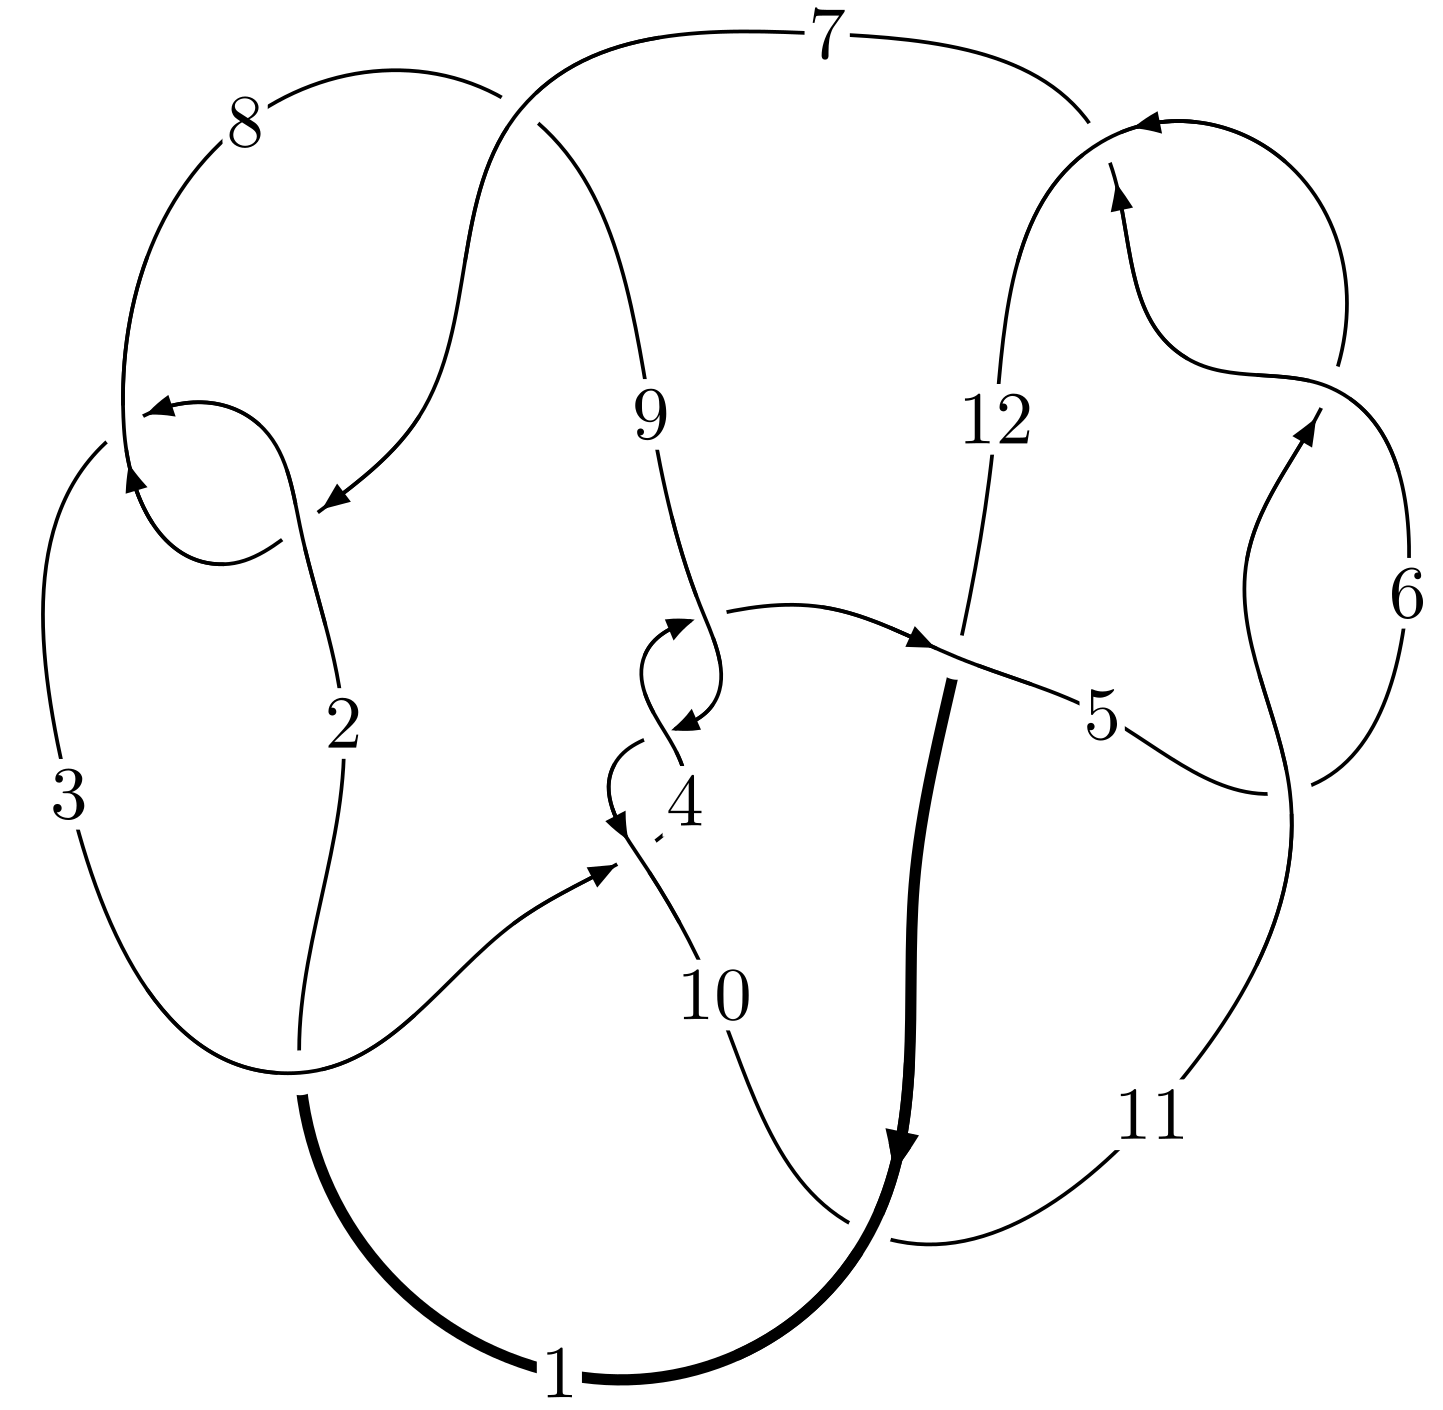
\includegraphics[width=112pt]{../../../GIT/diagram.site/Diagrams/png/1549_12a_0748.png}\\
\ \ \ A knot diagram\footnotemark}&
\allowdisplaybreaks
\textbf{Linearized knot diagam} \\
\cline{2-2}
 &
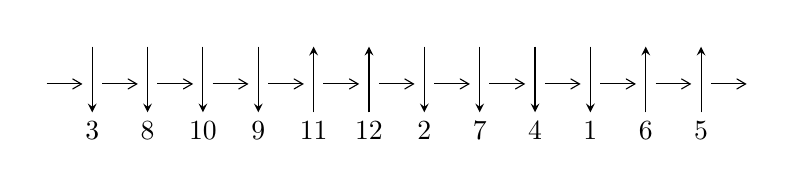
\begin{tikzpicture}[x=20pt, y=17pt]
	% nodes
	\node (C0) at (0, 0) {};
	\node (C1) at (1, 0) {};
	\node (C1U) at (1, +1) {};
	\node (C1D) at (1, -1) {3};

	\node (C2) at (2, 0) {};
	\node (C2U) at (2, +1) {};
	\node (C2D) at (2, -1) {8};

	\node (C3) at (3, 0) {};
	\node (C3U) at (3, +1) {};
	\node (C3D) at (3, -1) {10};

	\node (C4) at (4, 0) {};
	\node (C4U) at (4, +1) {};
	\node (C4D) at (4, -1) {9};

	\node (C5) at (5, 0) {};
	\node (C5U) at (5, +1) {};
	\node (C5D) at (5, -1) {11};

	\node (C6) at (6, 0) {};
	\node (C6U) at (6, +1) {};
	\node (C6D) at (6, -1) {12};

	\node (C7) at (7, 0) {};
	\node (C7U) at (7, +1) {};
	\node (C7D) at (7, -1) {2};

	\node (C8) at (8, 0) {};
	\node (C8U) at (8, +1) {};
	\node (C8D) at (8, -1) {7};

	\node (C9) at (9, 0) {};
	\node (C9U) at (9, +1) {};
	\node (C9D) at (9, -1) {4};

	\node (C10) at (10, 0) {};
	\node (C10U) at (10, +1) {};
	\node (C10D) at (10, -1) {1};

	\node (C11) at (11, 0) {};
	\node (C11U) at (11, +1) {};
	\node (C11D) at (11, -1) {6};

	\node (C12) at (12, 0) {};
	\node (C12U) at (12, +1) {};
	\node (C12D) at (12, -1) {5};
	\node (C13) at (13, 0) {};

	% arrows
	\draw[->,>={angle 60}]
	(C0) edge (C1) (C1) edge (C2) (C2) edge (C3) (C3) edge (C4) (C4) edge (C5) (C5) edge (C6) (C6) edge (C7) (C7) edge (C8) (C8) edge (C9) (C9) edge (C10) (C10) edge (C11) (C11) edge (C12) (C12) edge (C13) ;	\draw[->,>=stealth]
	(C1U) edge (C1D) (C2U) edge (C2D) (C3U) edge (C3D) (C4U) edge (C4D) (C5D) edge (C5U) (C6D) edge (C6U) (C7U) edge (C7D) (C8U) edge (C8D) (C9U) edge (C9D) (C10U) edge (C10D) (C11D) edge (C11U) (C12D) edge (C12U) ;
	\end{tikzpicture} \\
\hhline{~~} \\& 
\textbf{Solving Sequence} \\ \cline{2-2} 
 &
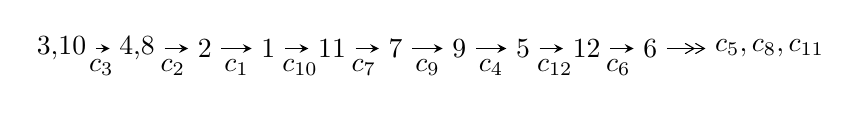
\begin{tikzpicture}[x=23pt, y=7pt]
	% node
	\node (A0) at (-1/8, 0) {3,10};
	\node (A1) at (17/16, 0) {4,8};
	\node (A2) at (17/8, 0) {2};
	\node (A3) at (25/8, 0) {1};
	\node (A4) at (33/8, 0) {11};
	\node (A5) at (41/8, 0) {7};
	\node (A6) at (49/8, 0) {9};
	\node (A7) at (57/8, 0) {5};
	\node (A8) at (65/8, 0) {12};
	\node (A9) at (73/8, 0) {6};
	\node (C1) at (1/2, -1) {$c_{3}$};
	\node (C2) at (13/8, -1) {$c_{2}$};
	\node (C3) at (21/8, -1) {$c_{1}$};
	\node (C4) at (29/8, -1) {$c_{10}$};
	\node (C5) at (37/8, -1) {$c_{7}$};
	\node (C6) at (45/8, -1) {$c_{9}$};
	\node (C7) at (53/8, -1) {$c_{4}$};
	\node (C8) at (61/8, -1) {$c_{12}$};
	\node (C9) at (69/8, -1) {$c_{6}$};
	\node (A10) at (11, 0) {$c_{5},c_{8},c_{11}$};

	% edge
	\draw[->,>=stealth]	
	(A0) edge (A1) (A1) edge (A2) (A2) edge (A3) (A3) edge (A4) (A4) edge (A5) (A5) edge (A6) (A6) edge (A7) (A7) edge (A8) (A8) edge (A9) ;
	\draw[->>,>={angle 60}]	
	(A9) edge (A10);
\end{tikzpicture} \\ 

\end{tabular} \\

\footnotetext{
The image of knot diagram is generated by the software ``\textbf{Draw programme}" developed by Andrew Bartholomew(\url{http://www.layer8.co.uk/maths/draw/index.htm\#Running-draw}), where we modified some parts for our purpose(\url{https://github.com/CATsTAILs/LinksPainter}).
}\phantom \\ \newline 
\centering \textbf{Ideals for irreducible components\footnotemark of $X_{\text{par}}$} 
 
\begin{align*}
I^u_{1}&=\langle 
-1.87140\times10^{123} u^{79}+2.18263\times10^{123} u^{78}+\cdots+7.17978\times10^{123} b-6.11537\times10^{123},\\
\phantom{I^u_{1}}&\phantom{= \langle  }-1.40244\times10^{124} u^{79}+1.63676\times10^{124} u^{78}+\cdots+7.17978\times10^{123} a-6.01317\times10^{124},\\
\phantom{I^u_{1}}&\phantom{= \langle  }u^{80}- u^{79}+\cdots+14 u+1\rangle \\
I^u_{2}&=\langle 
- a^4 u- a^3 u-4 a^3+5 a^2 u-3 a^2+2 a u+b+2 a,\\
\phantom{I^u_{2}}&\phantom{= \langle  }a^6-6 a^5 u+a^5-5 a^4 u-14 a^4+16 a^3 u-8 a^3+4 a^2 u+10 a^2-4 a u- a+u,\;u^2+1\rangle \\
\\
\end{align*}
\raggedright * 2 irreducible components of $\dim_{\mathbb{C}}=0$, with total 92 representations.\\
\footnotetext{All coefficients of polynomials are rational numbers. But the coefficients are sometimes approximated in decimal forms when there is not enough margin.}
\newpage
\renewcommand{\arraystretch}{1}
\centering \section*{I. $I^u_{1}= \langle -1.87\times10^{123} u^{79}+2.18\times10^{123} u^{78}+\cdots+7.18\times10^{123} b-6.12\times10^{123},\;-1.40\times10^{124} u^{79}+1.64\times10^{124} u^{78}+\cdots+7.18\times10^{123} a-6.01\times10^{124},\;u^{80}- u^{79}+\cdots+14 u+1 \rangle$}
\flushleft \textbf{(i) Arc colorings}\\
\begin{tabular}{m{7pt} m{180pt} m{7pt} m{180pt} }
\flushright $a_{3}=$&$\begin{pmatrix}1\\0\end{pmatrix}$ \\
\flushright $a_{10}=$&$\begin{pmatrix}0\\u\end{pmatrix}$ \\
\flushright $a_{4}=$&$\begin{pmatrix}1\\u^2\end{pmatrix}$ \\
\flushright $a_{8}=$&$\begin{pmatrix}1.95331 u^{79}-2.27968 u^{78}+\cdots+136.278 u+8.37515\\0.260648 u^{79}-0.303997 u^{78}+\cdots+19.3110 u+0.851748\end{pmatrix}$ \\
\flushright $a_{2}=$&$\begin{pmatrix}1.49413 u^{79}-1.06018 u^{78}+\cdots+149.804 u+16.0944\\0.0909719 u^{79}-0.306689 u^{78}+\cdots+10.2215 u+0.390652\end{pmatrix}$ \\
\flushright $a_{1}=$&$\begin{pmatrix}1.58510 u^{79}-1.36687 u^{78}+\cdots+160.025 u+16.4850\\0.0909719 u^{79}-0.306689 u^{78}+\cdots+10.2215 u+0.390652\end{pmatrix}$ \\
\flushright $a_{11}=$&$\begin{pmatrix}2.28061 u^{79}-2.53229 u^{78}+\cdots+165.250 u+9.03889\\0.337528 u^{79}-0.365997 u^{78}+\cdots+17.0768 u+0.443473\end{pmatrix}$ \\
\flushright $a_{7}=$&$\begin{pmatrix}0.824595 u^{79}-0.983888 u^{78}+\cdots+28.2566 u-6.24653\\-0.133058 u^{79}+0.0689018 u^{78}+\cdots-3.41790 u-1.33483\end{pmatrix}$ \\
\flushright $a_{9}=$&$\begin{pmatrix}u\\u^3+u\end{pmatrix}$ \\
\flushright $a_{5}=$&$\begin{pmatrix}u^2+1\\u^4+2 u^2\end{pmatrix}$ \\
\flushright $a_{12}=$&$\begin{pmatrix}1.41068 u^{79}-0.973288 u^{78}+\cdots+145.197 u+15.9700\\0.0510447 u^{79}-0.267505 u^{78}+\cdots+9.59013 u+0.315140\end{pmatrix}$ \\
\flushright $a_{6}=$&$\begin{pmatrix}2.87903 u^{79}-3.41840 u^{78}+\cdots+217.745 u+15.4041\\0.279564 u^{79}-0.233512 u^{78}+\cdots+21.0602 u+0.435870\end{pmatrix}$\\&\end{tabular}
\flushleft \textbf{(ii) Obstruction class $= -1$}\\~\\
\flushleft \textbf{(iii) Cusp Shapes $= -0.928763 u^{79}+1.11812 u^{78}+\cdots-28.6561 u-6.34554$}\\~\\
\newpage\renewcommand{\arraystretch}{1}
\flushleft \textbf{(iv) u-Polynomials at the component}\newline \\
\begin{tabular}{m{50pt}|m{274pt}}
Crossings & \hspace{64pt}u-Polynomials at each crossing \\
\hline $$\begin{aligned}c_{1},c_{8}\end{aligned}$$&$\begin{aligned}
&u^{80}+25 u^{79}+\cdots+60 u+25
\end{aligned}$\\
\hline $$\begin{aligned}c_{2},c_{7}\end{aligned}$$&$\begin{aligned}
&u^{80}+u^{79}+\cdots-6 u^2+5
\end{aligned}$\\
\hline $$\begin{aligned}c_{3},c_{4},c_{9}\end{aligned}$$&$\begin{aligned}
&u^{80}+u^{79}+\cdots-14 u+1
\end{aligned}$\\
\hline $$\begin{aligned}c_{5},c_{6},c_{11}\end{aligned}$$&$\begin{aligned}
&u^{80}+u^{79}+\cdots-10 u+1
\end{aligned}$\\
\hline $$\begin{aligned}c_{10}\end{aligned}$$&$\begin{aligned}
&u^{80}-15 u^{79}+\cdots-39596 u+1033
\end{aligned}$\\
\hline $$\begin{aligned}c_{12}\end{aligned}$$&$\begin{aligned}
&u^{80}-3 u^{79}+\cdots+13830 u-989
\end{aligned}$\\
\hline
\end{tabular}\\~\\
\newpage\renewcommand{\arraystretch}{1}
\flushleft \textbf{(v) Riley Polynomials at the component}\newline \\
\begin{tabular}{m{50pt}|m{274pt}}
Crossings & \hspace{64pt}Riley Polynomials at each crossing \\
\hline $$\begin{aligned}c_{1},c_{8}\end{aligned}$$&$\begin{aligned}
&y^{80}+67 y^{79}+\cdots-50800 y+625
\end{aligned}$\\
\hline $$\begin{aligned}c_{2},c_{7}\end{aligned}$$&$\begin{aligned}
&y^{80}-25 y^{79}+\cdots-60 y+25
\end{aligned}$\\
\hline $$\begin{aligned}c_{3},c_{4},c_{9}\end{aligned}$$&$\begin{aligned}
&y^{80}+81 y^{79}+\cdots-18 y+1
\end{aligned}$\\
\hline $$\begin{aligned}c_{5},c_{6},c_{11}\end{aligned}$$&$\begin{aligned}
&y^{80}-75 y^{79}+\cdots-38 y+1
\end{aligned}$\\
\hline $$\begin{aligned}c_{10}\end{aligned}$$&$\begin{aligned}
&y^{80}+45 y^{79}+\cdots-124136878 y+1067089
\end{aligned}$\\
\hline $$\begin{aligned}c_{12}\end{aligned}$$&$\begin{aligned}
&y^{80}-15 y^{79}+\cdots-85902818 y+978121
\end{aligned}$\\
\hline
\end{tabular}\\~\\
\newpage\flushleft \textbf{(vi) Complex Volumes and Cusp Shapes}
$$\begin{array}{c|c|c}  
\text{Solutions to }I^u_{1}& \I (\text{vol} + \sqrt{-1}CS) & \text{Cusp shape}\\
 \hline 
\begin{aligned}
u &= \phantom{-}0.101733 + 0.978535 I \\
a &= -0.033701 + 1.093690 I \\
b &= -0.799435 - 0.496821 I\end{aligned}
 & \phantom{-}1.74572 - 2.06211 I & \phantom{-0.000000 } 0 \\ \hline\begin{aligned}
u &= \phantom{-}0.101733 - 0.978535 I \\
a &= -0.033701 - 1.093690 I \\
b &= -0.799435 + 0.496821 I\end{aligned}
 & \phantom{-}1.74572 + 2.06211 I & \phantom{-0.000000 } 0 \\ \hline\begin{aligned}
u &= \phantom{-}0.932168 + 0.451237 I \\
a &= -0.864775 + 1.096610 I \\
b &= -0.980241 - 0.768254 I\end{aligned}
 & \phantom{-}8.13397 - 10.72160 I & \phantom{-0.000000 } 0 \\ \hline\begin{aligned}
u &= \phantom{-}0.932168 - 0.451237 I \\
a &= -0.864775 - 1.096610 I \\
b &= -0.980241 + 0.768254 I\end{aligned}
 & \phantom{-}8.13397 + 10.72160 I & \phantom{-0.000000 } 0 \\ \hline\begin{aligned}
u &= -0.671867 + 0.691792 I \\
a &= \phantom{-}0.251308 + 0.385725 I \\
b &= -0.848915 - 0.748997 I\end{aligned}
 & \phantom{-}3.18517 - 2.17478 I & \phantom{-0.000000 } 0 \\ \hline\begin{aligned}
u &= -0.671867 - 0.691792 I \\
a &= \phantom{-}0.251308 - 0.385725 I \\
b &= -0.848915 + 0.748997 I\end{aligned}
 & \phantom{-}3.18517 + 2.17478 I & \phantom{-0.000000 } 0 \\ \hline\begin{aligned}
u &= -0.886988 + 0.540330 I \\
a &= \phantom{-}0.171370 + 0.233050 I \\
b &= -0.777836 - 0.830954 I\end{aligned}
 & \phantom{-}8.75856 + 4.73589 I & \phantom{-0.000000 } 0 \\ \hline\begin{aligned}
u &= -0.886988 - 0.540330 I \\
a &= \phantom{-}0.171370 - 0.233050 I \\
b &= -0.777836 + 0.830954 I\end{aligned}
 & \phantom{-}8.75856 - 4.73589 I & \phantom{-0.000000 } 0 \\ \hline\begin{aligned}
u &= -0.843750 + 0.446002 I \\
a &= \phantom{-}0.86480 + 1.19833 I \\
b &= \phantom{-}0.959903 - 0.744068 I\end{aligned}
 & \phantom{-}2.34197 + 7.34848 I & \phantom{-0.000000 } 0 \\ \hline\begin{aligned}
u &= -0.843750 - 0.446002 I \\
a &= \phantom{-}0.86480 - 1.19833 I \\
b &= \phantom{-}0.959903 + 0.744068 I\end{aligned}
 & \phantom{-}2.34197 - 7.34848 I & \phantom{-0.000000 } 0\\
 \hline 
 \end{array}$$\newpage$$\begin{array}{c|c|c}  
\text{Solutions to }I^u_{1}& \I (\text{vol} + \sqrt{-1}CS) & \text{Cusp shape}\\
 \hline 
\begin{aligned}
u &= \phantom{-}0.773404 + 0.533895 I \\
a &= -0.243368 + 0.246513 I \\
b &= \phantom{-}0.781008 - 0.781882 I\end{aligned}
 & \phantom{-}2.88709 - 1.58183 I & \phantom{-0.000000 } 0 \\ \hline\begin{aligned}
u &= \phantom{-}0.773404 - 0.533895 I \\
a &= -0.243368 - 0.246513 I \\
b &= \phantom{-}0.781008 + 0.781882 I\end{aligned}
 & \phantom{-}2.88709 + 1.58183 I & \phantom{-0.000000 } 0 \\ \hline\begin{aligned}
u &= \phantom{-}0.211758 + 1.045890 I \\
a &= \phantom{-}0.01122 + 1.50037 I \\
b &= -0.625781 + 0.073783 I\end{aligned}
 & \phantom{-}4.13037 + 3.00225 I & \phantom{-0.000000 } 0 \\ \hline\begin{aligned}
u &= \phantom{-}0.211758 - 1.045890 I \\
a &= \phantom{-}0.01122 - 1.50037 I \\
b &= -0.625781 - 0.073783 I\end{aligned}
 & \phantom{-}4.13037 - 3.00225 I & \phantom{-0.000000 } 0 \\ \hline\begin{aligned}
u &= -0.820630 + 0.689518 I \\
a &= \phantom{-}0.610056 + 1.148510 I \\
b &= \phantom{-}0.885344 - 0.795442 I\end{aligned}
 & \phantom{-}9.21149 + 1.01170 I & \phantom{-0.000000 } 0 \\ \hline\begin{aligned}
u &= -0.820630 - 0.689518 I \\
a &= \phantom{-}0.610056 - 1.148510 I \\
b &= \phantom{-}0.885344 + 0.795442 I\end{aligned}
 & \phantom{-}9.21149 - 1.01170 I & \phantom{-0.000000 } 0 \\ \hline\begin{aligned}
u &= \phantom{-}0.732575 + 0.554489 I \\
a &= -0.69837 + 1.29546 I \\
b &= -0.905606 - 0.738630 I\end{aligned}
 & \phantom{-}3.00895 - 3.47648 I & \phantom{-0.000000 } 0 \\ \hline\begin{aligned}
u &= \phantom{-}0.732575 - 0.554489 I \\
a &= -0.69837 - 1.29546 I \\
b &= -0.905606 + 0.738630 I\end{aligned}
 & \phantom{-}3.00895 + 3.47648 I & \phantom{-0.000000 } 0 \\ \hline\begin{aligned}
u &= -0.218430 + 1.086470 I \\
a &= \phantom{-}0.214726 + 1.351440 I \\
b &= \phantom{-}0.730735 - 0.049838 I\end{aligned}
 & -0.492772 + 0.251831 I & \phantom{-0.000000 } 0 \\ \hline\begin{aligned}
u &= -0.218430 - 1.086470 I \\
a &= \phantom{-}0.214726 - 1.351440 I \\
b &= \phantom{-}0.730735 + 0.049838 I\end{aligned}
 & -0.492772 - 0.251831 I & \phantom{-0.000000 } 0\\
 \hline 
 \end{array}$$\newpage$$\begin{array}{c|c|c}  
\text{Solutions to }I^u_{1}& \I (\text{vol} + \sqrt{-1}CS) & \text{Cusp shape}\\
 \hline 
\begin{aligned}
u &= \phantom{-}0.775030 + 0.799999 I \\
a &= -0.154885 + 0.388889 I \\
b &= \phantom{-}0.889389 - 0.791856 I\end{aligned}
 & \phantom{-}9.19741 + 4.94494 I & \phantom{-0.000000 } 0 \\ \hline\begin{aligned}
u &= \phantom{-}0.775030 - 0.799999 I \\
a &= -0.154885 - 0.388889 I \\
b &= \phantom{-}0.889389 + 0.791856 I\end{aligned}
 & \phantom{-}9.19741 - 4.94494 I & \phantom{-0.000000 } 0 \\ \hline\begin{aligned}
u &= -0.362426 + 1.100800 I \\
a &= \phantom{-}0.165931 + 1.100420 I \\
b &= \phantom{-}0.583672 - 0.661495 I\end{aligned}
 & \phantom{-}6.51022 + 2.68209 I & \phantom{-0.000000 } 0 \\ \hline\begin{aligned}
u &= -0.362426 - 1.100800 I \\
a &= \phantom{-}0.165931 - 1.100420 I \\
b &= \phantom{-}0.583672 + 0.661495 I\end{aligned}
 & \phantom{-}6.51022 - 2.68209 I & \phantom{-0.000000 } 0 \\ \hline\begin{aligned}
u &= \phantom{-}0.295810 + 1.134100 I \\
a &= -0.003573 + 0.715062 I \\
b &= \phantom{-}1.001540 - 0.585236 I\end{aligned}
 & \phantom{-}5.23659 + 2.17110 I & \phantom{-0.000000 } 0 \\ \hline\begin{aligned}
u &= \phantom{-}0.295810 - 1.134100 I \\
a &= -0.003573 - 0.715062 I \\
b &= \phantom{-}1.001540 + 0.585236 I\end{aligned}
 & \phantom{-}5.23659 - 2.17110 I & \phantom{-0.000000 } 0 \\ \hline\begin{aligned}
u &= \phantom{-}0.241057 + 1.170000 I \\
a &= -0.414456 + 1.145130 I \\
b &= -0.921127 - 0.116588 I\end{aligned}
 & \phantom{-}2.45641 - 3.21481 I & \phantom{-0.000000 } 0 \\ \hline\begin{aligned}
u &= \phantom{-}0.241057 - 1.170000 I \\
a &= -0.414456 - 1.145130 I \\
b &= -0.921127 + 0.116588 I\end{aligned}
 & \phantom{-}2.45641 + 3.21481 I & \phantom{-0.000000 } 0 \\ \hline\begin{aligned}
u &= -0.345580 + 0.634269 I \\
a &= -0.285955 + 0.408231 I \\
b &= \phantom{-}0.015644 + 0.475314 I\end{aligned}
 & \phantom{-}4.83976 + 3.51631 I & \phantom{-}3.10687 - 4.94951 I \\ \hline\begin{aligned}
u &= -0.345580 - 0.634269 I \\
a &= -0.285955 - 0.408231 I \\
b &= \phantom{-}0.015644 - 0.475314 I\end{aligned}
 & \phantom{-}4.83976 - 3.51631 I & \phantom{-}3.10687 + 4.94951 I\\
 \hline 
 \end{array}$$\newpage$$\begin{array}{c|c|c}  
\text{Solutions to }I^u_{1}& \I (\text{vol} + \sqrt{-1}CS) & \text{Cusp shape}\\
 \hline 
\begin{aligned}
u &= \phantom{-}0.054082 + 1.332890 I \\
a &= -0.282249 + 0.830000 I \\
b &= -1.074650 - 0.347834 I\end{aligned}
 & \phantom{-}2.46046 - 1.87752 I & \phantom{-0.000000 } 0 \\ \hline\begin{aligned}
u &= \phantom{-}0.054082 - 1.332890 I \\
a &= -0.282249 - 0.830000 I \\
b &= -1.074650 + 0.347834 I\end{aligned}
 & \phantom{-}2.46046 + 1.87752 I & \phantom{-0.000000 } 0 \\ \hline\begin{aligned}
u &= \phantom{-}0.640087\phantom{ +0.000000I} \\
a &= \phantom{-}1.64399\phantom{ +0.000000I} \\
b &= \phantom{-}0.964662\phantom{ +0.000000I}\end{aligned}
 & -1.04598\phantom{ +0.000000I} & -8.67610\phantom{ +0.000000I} \\ \hline\begin{aligned}
u &= \phantom{-}0.575302 + 0.268375 I \\
a &= \phantom{-}1.99533 + 0.24230 I \\
b &= \phantom{-}0.981751 + 0.220824 I\end{aligned}
 & \phantom{-}1.92420 - 6.00380 I & -5.29609 + 7.13833 I \\ \hline\begin{aligned}
u &= \phantom{-}0.575302 - 0.268375 I \\
a &= \phantom{-}1.99533 - 0.24230 I \\
b &= \phantom{-}0.981751 - 0.220824 I\end{aligned}
 & \phantom{-}1.92420 + 6.00380 I & -5.29609 - 7.13833 I \\ \hline\begin{aligned}
u &= -0.588746 + 0.173171 I \\
a &= -1.77796 + 0.22741 I \\
b &= -0.955476 + 0.155992 I\end{aligned}
 & -3.12955 + 2.80147 I & -11.11475 - 6.33047 I \\ \hline\begin{aligned}
u &= -0.588746 - 0.173171 I \\
a &= -1.77796 - 0.22741 I \\
b &= -0.955476 - 0.155992 I\end{aligned}
 & -3.12955 - 2.80147 I & -11.11475 + 6.33047 I \\ \hline\begin{aligned}
u &= -0.174397 + 1.383230 I \\
a &= \phantom{-}0.400952 + 0.826741 I \\
b &= \phantom{-}1.125090 - 0.254913 I\end{aligned}
 & \phantom{-}1.83502 + 5.48427 I & \phantom{-0.000000 } 0 \\ \hline\begin{aligned}
u &= -0.174397 - 1.383230 I \\
a &= \phantom{-}0.400952 - 0.826741 I \\
b &= \phantom{-}1.125090 + 0.254913 I\end{aligned}
 & \phantom{-}1.83502 - 5.48427 I & \phantom{-0.000000 } 0 \\ \hline\begin{aligned}
u &= -0.04414 + 1.42255 I \\
a &= \phantom{-}0.93098 - 2.08220 I \\
b &= -0.881041 + 0.761522 I\end{aligned}
 & \phantom{-}4.02110 + 2.87995 I & \phantom{-0.000000 } 0\\
 \hline 
 \end{array}$$\newpage$$\begin{array}{c|c|c}  
\text{Solutions to }I^u_{1}& \I (\text{vol} + \sqrt{-1}CS) & \text{Cusp shape}\\
 \hline 
\begin{aligned}
u &= -0.04414 - 1.42255 I \\
a &= \phantom{-}0.93098 + 2.08220 I \\
b &= -0.881041 - 0.761522 I\end{aligned}
 & \phantom{-}4.02110 - 2.87995 I & \phantom{-0.000000 } 0 \\ \hline\begin{aligned}
u &= -0.03050 + 1.42320 I \\
a &= -1.17424 - 1.79296 I \\
b &= \phantom{-}0.836814 + 0.773435 I\end{aligned}
 & \phantom{-}7.88157 + 1.28407 I & \phantom{-0.000000 } 0 \\ \hline\begin{aligned}
u &= -0.03050 - 1.42320 I \\
a &= -1.17424 + 1.79296 I \\
b &= \phantom{-}0.836814 - 0.773435 I\end{aligned}
 & \phantom{-}7.88157 - 1.28407 I & \phantom{-0.000000 } 0 \\ \hline\begin{aligned}
u &= \phantom{-}0.11860 + 1.43036 I \\
a &= -0.58859 - 2.23064 I \\
b &= \phantom{-}0.924105 + 0.756075 I\end{aligned}
 & \phantom{-}7.61249 - 7.06523 I & \phantom{-0.000000 } 0 \\ \hline\begin{aligned}
u &= \phantom{-}0.11860 - 1.43036 I \\
a &= -0.58859 + 2.23064 I \\
b &= \phantom{-}0.924105 - 0.756075 I\end{aligned}
 & \phantom{-}7.61249 + 7.06523 I & \phantom{-0.000000 } 0 \\ \hline\begin{aligned}
u &= \phantom{-}0.00024 + 1.44080 I \\
a &= \phantom{-}0.285840 + 0.736919 I \\
b &= \phantom{-}1.151750 - 0.388320 I\end{aligned}
 & \phantom{-}8.39629 - 0.63079 I & \phantom{-0.000000 } 0 \\ \hline\begin{aligned}
u &= \phantom{-}0.00024 - 1.44080 I \\
a &= \phantom{-}0.285840 - 0.736919 I \\
b &= \phantom{-}1.151750 + 0.388320 I\end{aligned}
 & \phantom{-}8.39629 + 0.63079 I & \phantom{-0.000000 } 0 \\ \hline\begin{aligned}
u &= \phantom{-}0.05174 + 1.45148 I \\
a &= -0.018131 + 0.962979 I \\
b &= -0.056374 - 0.795689 I\end{aligned}
 & \phantom{-}5.80702 - 1.98974 I & \phantom{-0.000000 } 0 \\ \hline\begin{aligned}
u &= \phantom{-}0.05174 - 1.45148 I \\
a &= -0.018131 - 0.962979 I \\
b &= -0.056374 + 0.795689 I\end{aligned}
 & \phantom{-}5.80702 + 1.98974 I & \phantom{-0.000000 } 0 \\ \hline\begin{aligned}
u &= \phantom{-}0.19387 + 1.44583 I \\
a &= -0.425784 + 0.774845 I \\
b &= -1.176240 - 0.252011 I\end{aligned}
 & \phantom{-}7.54244 - 8.76456 I & \phantom{-0.000000 } 0\\
 \hline 
 \end{array}$$\newpage$$\begin{array}{c|c|c}  
\text{Solutions to }I^u_{1}& \I (\text{vol} + \sqrt{-1}CS) & \text{Cusp shape}\\
 \hline 
\begin{aligned}
u &= \phantom{-}0.19387 - 1.44583 I \\
a &= -0.425784 - 0.774845 I \\
b &= -1.176240 + 0.252011 I\end{aligned}
 & \phantom{-}7.54244 + 8.76456 I & \phantom{-0.000000 } 0 \\ \hline\begin{aligned}
u &= \phantom{-}0.513658\phantom{ +0.000000I} \\
a &= \phantom{-}1.37806\phantom{ +0.000000I} \\
b &= \phantom{-}0.827741\phantom{ +0.000000I}\end{aligned}
 & -1.34189\phantom{ +0.000000I} & -6.91700\phantom{ +0.000000I} \\ \hline\begin{aligned}
u &= -0.507056 + 0.053892 I \\
a &= -0.002765 + 0.465935 I \\
b &= -0.517576 + 0.509108 I\end{aligned}
 & \phantom{-}3.24338 - 0.59067 I & -0.928629 - 0.584065 I \\ \hline\begin{aligned}
u &= -0.507056 - 0.053892 I \\
a &= -0.002765 - 0.465935 I \\
b &= -0.517576 - 0.509108 I\end{aligned}
 & \phantom{-}3.24338 + 0.59067 I & -0.928629 + 0.584065 I \\ \hline\begin{aligned}
u &= \phantom{-}0.476219 + 0.168968 I \\
a &= -1.43519 + 2.10419 I \\
b &= -0.942034 - 0.603774 I\end{aligned}
 & \phantom{-}2.30977 - 5.10729 I & -4.12064 + 6.77014 I \\ \hline\begin{aligned}
u &= \phantom{-}0.476219 - 0.168968 I \\
a &= -1.43519 - 2.10419 I \\
b &= -0.942034 + 0.603774 I\end{aligned}
 & \phantom{-}2.30977 + 5.10729 I & -4.12064 - 6.77014 I \\ \hline\begin{aligned}
u &= -0.09439 + 1.52168 I \\
a &= \phantom{-}0.031950 + 0.938149 I \\
b &= \phantom{-}0.091903 - 0.871946 I\end{aligned}
 & \phantom{-}11.90470 + 5.02795 I & \phantom{-0.000000 } 0 \\ \hline\begin{aligned}
u &= -0.09439 - 1.52168 I \\
a &= \phantom{-}0.031950 - 0.938149 I \\
b &= \phantom{-}0.091903 + 0.871946 I\end{aligned}
 & \phantom{-}11.90470 - 5.02795 I & \phantom{-0.000000 } 0 \\ \hline\begin{aligned}
u &= \phantom{-}0.257516 + 0.387955 I \\
a &= \phantom{-}0.161469 + 0.323631 I \\
b &= \phantom{-}0.107563 + 0.368320 I\end{aligned}
 & -0.128336 - 1.019230 I & -2.35092 + 6.58230 I \\ \hline\begin{aligned}
u &= \phantom{-}0.257516 - 0.387955 I \\
a &= \phantom{-}0.161469 - 0.323631 I \\
b &= \phantom{-}0.107563 - 0.368320 I\end{aligned}
 & -0.128336 + 1.019230 I & -2.35092 - 6.58230 I\\
 \hline 
 \end{array}$$\newpage$$\begin{array}{c|c|c}  
\text{Solutions to }I^u_{1}& \I (\text{vol} + \sqrt{-1}CS) & \text{Cusp shape}\\
 \hline 
\begin{aligned}
u &= \phantom{-}0.25346 + 1.52819 I \\
a &= -0.03652 - 1.93780 I \\
b &= \phantom{-}1.007120 + 0.789658 I\end{aligned}
 & \phantom{-}9.78276 - 7.07394 I & \phantom{-0.000000 } 0 \\ \hline\begin{aligned}
u &= \phantom{-}0.25346 - 1.52819 I \\
a &= -0.03652 + 1.93780 I \\
b &= \phantom{-}1.007120 - 0.789658 I\end{aligned}
 & \phantom{-}9.78276 + 7.07394 I & \phantom{-0.000000 } 0 \\ \hline\begin{aligned}
u &= -0.31104 + 1.51921 I \\
a &= -0.13083 - 1.93728 I \\
b &= -1.034310 + 0.777789 I\end{aligned}
 & \phantom{-}8.7210 + 11.5709 I & \phantom{-0.000000 } 0 \\ \hline\begin{aligned}
u &= -0.31104 - 1.51921 I \\
a &= -0.13083 + 1.93728 I \\
b &= -1.034310 - 0.777789 I\end{aligned}
 & \phantom{-}8.7210 - 11.5709 I & \phantom{-0.000000 } 0 \\ \hline\begin{aligned}
u &= -0.19543 + 1.54802 I \\
a &= -0.92101 - 1.11661 I \\
b &= \phantom{-}0.766788 + 0.884790 I\end{aligned}
 & \phantom{-}10.53440 + 0.86706 I & \phantom{-0.000000 } 0 \\ \hline\begin{aligned}
u &= -0.19543 - 1.54802 I \\
a &= -0.92101 + 1.11661 I \\
b &= \phantom{-}0.766788 - 0.884790 I\end{aligned}
 & \phantom{-}10.53440 - 0.86706 I & \phantom{-0.000000 } 0 \\ \hline\begin{aligned}
u &= \phantom{-}0.26150 + 1.53905 I \\
a &= \phantom{-}0.933999 - 0.963161 I \\
b &= -0.726409 + 0.898691 I\end{aligned}
 & \phantom{-}9.68026 - 5.36620 I & \phantom{-0.000000 } 0 \\ \hline\begin{aligned}
u &= \phantom{-}0.26150 - 1.53905 I \\
a &= \phantom{-}0.933999 + 0.963161 I \\
b &= -0.726409 - 0.898691 I\end{aligned}
 & \phantom{-}9.68026 + 5.36620 I & \phantom{-0.000000 } 0 \\ \hline\begin{aligned}
u &= \phantom{-}0.34836 + 1.53663 I \\
a &= \phantom{-}0.21307 - 1.86398 I \\
b &= \phantom{-}1.054520 + 0.781483 I\end{aligned}
 & \phantom{-}14.5640 - 15.3956 I & \phantom{-0.000000 } 0 \\ \hline\begin{aligned}
u &= \phantom{-}0.34836 - 1.53663 I \\
a &= \phantom{-}0.21307 + 1.86398 I \\
b &= \phantom{-}1.054520 - 0.781483 I\end{aligned}
 & \phantom{-}14.5640 + 15.3956 I & \phantom{-0.000000 } 0\\
 \hline 
 \end{array}$$\newpage$$\begin{array}{c|c|c}  
\text{Solutions to }I^u_{1}& \I (\text{vol} + \sqrt{-1}CS) & \text{Cusp shape}\\
 \hline 
\begin{aligned}
u &= -0.30441 + 1.56366 I \\
a &= -0.868025 - 0.886761 I \\
b &= \phantom{-}0.709930 + 0.925967 I\end{aligned}
 & \phantom{-}15.6429 + 9.1022 I & \phantom{-0.000000 } 0 \\ \hline\begin{aligned}
u &= -0.30441 - 1.56366 I \\
a &= -0.868025 + 0.886761 I \\
b &= \phantom{-}0.709930 - 0.925967 I\end{aligned}
 & \phantom{-}15.6429 - 9.1022 I & \phantom{-0.000000 } 0 \\ \hline\begin{aligned}
u &= -0.22395 + 1.60407 I \\
a &= \phantom{-}0.11170 - 1.73571 I \\
b &= -1.003300 + 0.831540 I\end{aligned}
 & \phantom{-}16.9165 + 4.8171 I & \phantom{-0.000000 } 0 \\ \hline\begin{aligned}
u &= -0.22395 - 1.60407 I \\
a &= \phantom{-}0.11170 + 1.73571 I \\
b &= -1.003300 - 0.831540 I\end{aligned}
 & \phantom{-}16.9165 - 4.8171 I & \phantom{-0.000000 } 0 \\ \hline\begin{aligned}
u &= \phantom{-}0.16076 + 1.62447 I \\
a &= \phantom{-}0.741747 - 1.164460 I \\
b &= -0.806249 + 0.918049 I\end{aligned}
 & \phantom{-}17.5372 + 1.6269 I & \phantom{-0.000000 } 0 \\ \hline\begin{aligned}
u &= \phantom{-}0.16076 - 1.62447 I \\
a &= \phantom{-}0.741747 + 1.164460 I \\
b &= -0.806249 - 0.918049 I\end{aligned}
 & \phantom{-}17.5372 - 1.6269 I & \phantom{-0.000000 } 0 \\ \hline\begin{aligned}
u &= -0.178705 + 0.120060 I \\
a &= \phantom{-}0.93450 + 4.97190 I \\
b &= \phantom{-}0.890770 - 0.549646 I\end{aligned}
 & -1.16657 + 2.14399 I & -10.37179 - 2.91834 I \\ \hline\begin{aligned}
u &= -0.178705 - 0.120060 I \\
a &= \phantom{-}0.93450 - 4.97190 I \\
b &= \phantom{-}0.890770 + 0.549646 I\end{aligned}
 & -1.16657 - 2.14399 I & -10.37179 + 2.91834 I \\ \hline\begin{aligned}
u &= -0.0896155 + 0.0906026 I \\
a &= -3.68162 + 6.94609 I \\
b &= -0.858957 + 0.460685 I\end{aligned}
 & \phantom{-}3.02062 - 0.76923 I & -4.51577 - 0.70346 I \\ \hline\begin{aligned}
u &= -0.0896155 - 0.0906026 I \\
a &= -3.68162 - 6.94609 I \\
b &= -0.858957 - 0.460685 I\end{aligned}
 & \phantom{-}3.02062 + 0.76923 I & -4.51577 + 0.70346 I\\
 \hline 
 \end{array}$$\newpage\newpage\renewcommand{\arraystretch}{1}
\centering \section*{II. $I^u_{2}= \langle - a^4 u- a^3 u+\cdots-3 a^2+2 a,\;-6 a^5 u-5 a^4 u+\cdots+10 a^2- a,\;u^2+1 \rangle$}
\flushleft \textbf{(i) Arc colorings}\\
\begin{tabular}{m{7pt} m{180pt} m{7pt} m{180pt} }
\flushright $a_{3}=$&$\begin{pmatrix}1\\0\end{pmatrix}$ \\
\flushright $a_{10}=$&$\begin{pmatrix}0\\u\end{pmatrix}$ \\
\flushright $a_{4}=$&$\begin{pmatrix}1\\-1\end{pmatrix}$ \\
\flushright $a_{8}=$&$\begin{pmatrix}a\\a^4 u+a^3 u+4 a^3-5 a^2 u+3 a^2-2 a u-2 a\end{pmatrix}$ \\
\flushright $a_{2}=$&$\begin{pmatrix}- a^5 u- a^4 u-4 a^4+5 a^3 u-3 a^3+2 a^2 u+2 a^2+1\\- a^4+4 a^3 u- a^3+3 a^2 u+5 a^2-2 a u+2 a-1\end{pmatrix}$ \\
\flushright $a_{1}=$&$\begin{pmatrix}- a^5 u- a^4 u-5 a^4+9 a^3 u-4 a^3+5 a^2 u+7 a^2-2 a u+2 a\\- a^4+4 a^3 u- a^3+3 a^2 u+5 a^2-2 a u+2 a-1\end{pmatrix}$ \\
\flushright $a_{11}=$&$\begin{pmatrix}a^3 u+3 a^2-3 a u+u-1\\- a+2 u\end{pmatrix}$ \\
\flushright $a_{7}=$&$\begin{pmatrix}- a^5+5 a^4 u- a^4+4 a^3 u+9 a^3-7 a^2 u+5 a^2-2 a u-2 a\\a^4 u+a^3 u+4 a^3-5 a^2 u+3 a^2-2 a u-2 a+u\end{pmatrix}$ \\
\flushright $a_{9}=$&$\begin{pmatrix}u\\0\end{pmatrix}$ \\
\flushright $a_{5}=$&$\begin{pmatrix}0\\-1\end{pmatrix}$ \\
\flushright $a_{12}=$&$\begin{pmatrix}- a^5 u- a^4 u-5 a^4+9 a^3 u-4 a^3+5 a^2 u+7 a^2-2 a u+2 a\\- a^5 u- a^4 u-6 a^4+13 a^3 u-5 a^3+8 a^2 u+12 a^2-4 a u+4 a-1\end{pmatrix}$ \\
\flushright $a_{6}=$&$\begin{pmatrix}- a^5+5 a^4 u- a^4+4 a^3 u+10 a^3-10 a^2 u+5 a^2-2 a u-5 a+u\\a^4 u+5 a^3-9 a^2 u+a u-7 a+2 u+1\end{pmatrix}$\\&\end{tabular}
\flushleft \textbf{(ii) Obstruction class $= 1$}\\~\\
\flushleft \textbf{(iii) Cusp Shapes $= 4 a^5-20 a^4 u+8 a^4-32 a^3 u-32 a^3+16 a^2 u-40 a^2+16 a u$}\\~\\
\newpage\renewcommand{\arraystretch}{1}
\flushleft \textbf{(iv) u-Polynomials at the component}\newline \\
\begin{tabular}{m{50pt}|m{274pt}}
Crossings & \hspace{64pt}u-Polynomials at each crossing \\
\hline $$\begin{aligned}c_{1}\end{aligned}$$&$\begin{aligned}
&(u^2- u+1)^6
\end{aligned}$\\
\hline $$\begin{aligned}c_{2},c_{7}\end{aligned}$$&$\begin{aligned}
&(u^4- u^2+1)^3
\end{aligned}$\\
\hline $$\begin{aligned}c_{3},c_{4},c_{9}\end{aligned}$$&$\begin{aligned}
&(u^2+1)^6
\end{aligned}$\\
\hline $$\begin{aligned}c_{5},c_{6},c_{11}\end{aligned}$$&$\begin{aligned}
&(u^6-3 u^4+2 u^2+1)^2
\end{aligned}$\\
\hline $$\begin{aligned}c_{8}\end{aligned}$$&$\begin{aligned}
&(u^2+u+1)^6
\end{aligned}$\\
\hline $$\begin{aligned}c_{10}\end{aligned}$$&$\begin{aligned}
&(u^3+u^2-1)^4
\end{aligned}$\\
\hline $$\begin{aligned}c_{12}\end{aligned}$$&$\begin{aligned}
&(u^6+u^4+2 u^2+1)^2
\end{aligned}$\\
\hline
\end{tabular}\\~\\
\newpage\renewcommand{\arraystretch}{1}
\flushleft \textbf{(v) Riley Polynomials at the component}\newline \\
\begin{tabular}{m{50pt}|m{274pt}}
Crossings & \hspace{64pt}Riley Polynomials at each crossing \\
\hline $$\begin{aligned}c_{1},c_{8}\end{aligned}$$&$\begin{aligned}
&(y^2+y+1)^6
\end{aligned}$\\
\hline $$\begin{aligned}c_{2},c_{7}\end{aligned}$$&$\begin{aligned}
&(y^2- y+1)^6
\end{aligned}$\\
\hline $$\begin{aligned}c_{3},c_{4},c_{9}\end{aligned}$$&$\begin{aligned}
&(y+1)^{12}
\end{aligned}$\\
\hline $$\begin{aligned}c_{5},c_{6},c_{11}\end{aligned}$$&$\begin{aligned}
&(y^3-3 y^2+2 y+1)^4
\end{aligned}$\\
\hline $$\begin{aligned}c_{10}\end{aligned}$$&$\begin{aligned}
&(y^3- y^2+2 y-1)^4
\end{aligned}$\\
\hline $$\begin{aligned}c_{12}\end{aligned}$$&$\begin{aligned}
&(y^3+y^2+2 y+1)^4
\end{aligned}$\\
\hline
\end{tabular}\\~\\
\newpage\flushleft \textbf{(vi) Complex Volumes and Cusp Shapes}
$$\begin{array}{c|c|c}  
\text{Solutions to }I^u_{2}& \I (\text{vol} + \sqrt{-1}CS) & \text{Cusp shape}\\
 \hline 
\begin{aligned}
u &= \phantom{-0.000000 -}1.000000 I \\
a &= -1.083790 + 0.612547 I \\
b &= -0.866025 - 0.500000 I\end{aligned}
 & \phantom{-}4.66906 + 0.79824 I & \phantom{-}1.50976 + 0.48465 I \\ \hline\begin{aligned}
u &= \phantom{-0.000000 -}1.000000 I \\
a &= \phantom{-}0.377439 + 0.346257 I \\
b &= \phantom{-}0.866025 - 0.500000 I\end{aligned}
 & \phantom{-}0.53148 + 2.02988 I & -5.01951 - 3.46410 I \\ \hline\begin{aligned}
u &= \phantom{-0.000000 -}1.000000 I \\
a &= \phantom{-}0.37744 + 1.65374 I \\
b &= -0.866025 - 0.500000 I\end{aligned}
 & \phantom{-}0.53148 - 2.02988 I & -5.01951 + 3.46410 I \\ \hline\begin{aligned}
u &= \phantom{-0.000000 -}1.000000 I \\
a &= \phantom{-}0.206350 - 0.132315 I \\
b &= -0.866025 - 0.500000 I\end{aligned}
 & \phantom{-}4.66906 - 4.85801 I & \phantom{-}1.50976 + 6.44355 I \\ \hline\begin{aligned}
u &= \phantom{-0.000000 -}1.000000 I \\
a &= -1.08379 + 1.38745 I \\
b &= \phantom{-}0.866025 - 0.500000 I\end{aligned}
 & \phantom{-}4.66906 - 0.79824 I & \phantom{-}1.50976 - 0.48465 I \\ \hline\begin{aligned}
u &= \phantom{-0.000000 -}1.000000 I \\
a &= \phantom{-}0.20635 + 2.13232 I \\
b &= \phantom{-}0.866025 - 0.500000 I\end{aligned}
 & \phantom{-}4.66906 + 4.85801 I & \phantom{-}1.50976 - 6.44355 I \\ \hline\begin{aligned}
u &= \phantom{-0.000000 } -1.000000 I \\
a &= -1.083790 - 0.612547 I \\
b &= -0.866025 + 0.500000 I\end{aligned}
 & \phantom{-}4.66906 - 0.79824 I & \phantom{-}1.50976 - 0.48465 I \\ \hline\begin{aligned}
u &= \phantom{-0.000000 } -1.000000 I \\
a &= \phantom{-}0.377439 - 0.346257 I \\
b &= \phantom{-}0.866025 + 0.500000 I\end{aligned}
 & \phantom{-}0.53148 - 2.02988 I & -5.01951 + 3.46410 I \\ \hline\begin{aligned}
u &= \phantom{-0.000000 } -1.000000 I \\
a &= \phantom{-}0.37744 - 1.65374 I \\
b &= -0.866025 + 0.500000 I\end{aligned}
 & \phantom{-}0.53148 + 2.02988 I & -5.01951 - 3.46410 I \\ \hline\begin{aligned}
u &= \phantom{-0.000000 } -1.000000 I \\
a &= \phantom{-}0.206350 + 0.132315 I \\
b &= -0.866025 + 0.500000 I\end{aligned}
 & \phantom{-}4.66906 + 4.85801 I & \phantom{-}1.50976 - 6.44355 I\\
 \hline 
 \end{array}$$\newpage$$\begin{array}{c|c|c}  
\text{Solutions to }I^u_{2}& \I (\text{vol} + \sqrt{-1}CS) & \text{Cusp shape}\\
 \hline 
\begin{aligned}
u &= \phantom{-0.000000 } -1.000000 I \\
a &= -1.08379 - 1.38745 I \\
b &= \phantom{-}0.866025 + 0.500000 I\end{aligned}
 & \phantom{-}4.66906 + 0.79824 I & \phantom{-}1.50976 + 0.48465 I \\ \hline\begin{aligned}
u &= \phantom{-0.000000 } -1.000000 I \\
a &= \phantom{-}0.20635 - 2.13232 I \\
b &= \phantom{-}0.866025 + 0.500000 I\end{aligned}
 & \phantom{-}4.66906 - 4.85801 I & \phantom{-}1.50976 + 6.44355 I\\
 \hline 
 \end{array}$$\newpage
\newpage\renewcommand{\arraystretch}{1}
\centering \section*{ III. u-Polynomials}
\begin{tabular}{m{50pt}|m{274pt}}
Crossings & \hspace{64pt}u-Polynomials at each crossing \\
\hline $$\begin{aligned}c_{1}\end{aligned}$$&$\begin{aligned}
&((u^2- u+1)^6)(u^{80}+25 u^{79}+\cdots+60 u+25)
\end{aligned}$\\
\hline $$\begin{aligned}c_{2},c_{7}\end{aligned}$$&$\begin{aligned}
&((u^4- u^2+1)^3)(u^{80}+u^{79}+\cdots-6 u^2+5)
\end{aligned}$\\
\hline $$\begin{aligned}c_{3},c_{4},c_{9}\end{aligned}$$&$\begin{aligned}
&((u^2+1)^6)(u^{80}+u^{79}+\cdots-14 u+1)
\end{aligned}$\\
\hline $$\begin{aligned}c_{5},c_{6},c_{11}\end{aligned}$$&$\begin{aligned}
&((u^6-3 u^4+2 u^2+1)^2)(u^{80}+u^{79}+\cdots-10 u+1)
\end{aligned}$\\
\hline $$\begin{aligned}c_{8}\end{aligned}$$&$\begin{aligned}
&((u^2+u+1)^6)(u^{80}+25 u^{79}+\cdots+60 u+25)
\end{aligned}$\\
\hline $$\begin{aligned}c_{10}\end{aligned}$$&$\begin{aligned}
&((u^3+u^2-1)^4)(u^{80}-15 u^{79}+\cdots-39596 u+1033)
\end{aligned}$\\
\hline $$\begin{aligned}c_{12}\end{aligned}$$&$\begin{aligned}
&((u^6+u^4+2 u^2+1)^2)(u^{80}-3 u^{79}+\cdots+13830 u-989)
\end{aligned}$\\
\hline
\end{tabular}\newpage\renewcommand{\arraystretch}{1}
\centering \section*{ IV. Riley Polynomials}
\begin{tabular}{m{50pt}|m{274pt}}
Crossings & \hspace{64pt}Riley Polynomials at each crossing \\
\hline $$\begin{aligned}c_{1},c_{8}\end{aligned}$$&$\begin{aligned}
&((y^2+y+1)^6)(y^{80}+67 y^{79}+\cdots-50800 y+625)
\end{aligned}$\\
\hline $$\begin{aligned}c_{2},c_{7}\end{aligned}$$&$\begin{aligned}
&((y^2- y+1)^6)(y^{80}-25 y^{79}+\cdots-60 y+25)
\end{aligned}$\\
\hline $$\begin{aligned}c_{3},c_{4},c_{9}\end{aligned}$$&$\begin{aligned}
&((y+1)^{12})(y^{80}+81 y^{79}+\cdots-18 y+1)
\end{aligned}$\\
\hline $$\begin{aligned}c_{5},c_{6},c_{11}\end{aligned}$$&$\begin{aligned}
&((y^3-3 y^2+2 y+1)^4)(y^{80}-75 y^{79}+\cdots-38 y+1)
\end{aligned}$\\
\hline $$\begin{aligned}c_{10}\end{aligned}$$&$\begin{aligned}
&((y^3- y^2+2 y-1)^4)(y^{80}+45 y^{79}+\cdots-1.24137\times10^{8} y+1067089)
\end{aligned}$\\
\hline $$\begin{aligned}c_{12}\end{aligned}$$&$\begin{aligned}
&((y^3+y^2+2 y+1)^4)(y^{80}-15 y^{79}+\cdots-8.59028\times10^{7} y+978121)
\end{aligned}$\\
\hline
\end{tabular}
\vskip 2pc
\end{document}